% Required packages in the main thesis preamble:
%\usepackage{amsmath,amssymb,bm,graphicx}

\chapter{Methodology}
\label{chap:methodology}

\section{Overview}
\label{sec:methodology-overview}

The proposed model is a Transformer variant whose tokens remain symmetric
positive-definite (SPD) covariance matrices.  Instead of flattening a trial
into one long Euclidean sequence, it preserves the temporal, spectral, and
anatomical axes and attends to them successively.  For a batch of trials, the
input is
\begin{equation}
    \bm{\mathcal X}
    =\left\{\bm X_{tfr}\right\}_{t=1,f=1,r=1}^{T,F,R}
    \in\left(\mathbb S_{++}^{d_0}\right)^{T\times F\times R},
    \qquad
    \operatorname{shape}(\bm{\mathcal X})
    =B\times T\times F\times R\times d_0\times d_0,
    \label{eq:overview-input}
\end{equation}
where $T$, $F$, and $R$ denote the numbers of temporal segments, frequency
bands, and brain regions, respectively.  With the main PhysioNet
configuration, a five-second epoch is divided into $T=19$ overlapping
$0.5\,$s windows, $F=3$ filter-bank bands and $R=8$ regions are used, and every
region contributes an $8\times8$ covariance matrix ($d_0=8$).

Figure~\ref{fig:spd-transformer-overview} summarises the end-to-end data flow.
The encoder retains the token-grid shape, produces interactions along each of
its three semantic axes, and returns symmetric log-domain representations of
the SPD tokens.  A
learned positional weighting then pools all tokens into one trial
representation, which is compared with learnable class prototypes by a
Log-Euclidean minimum-distance-to-mean (MDM) classifier.

\begin{figure}[t]
    \centering
    \IfFileExists{figures/spd_transformer_overview.pdf}{%
        \includegraphics[width=\textwidth]{figures/spd_transformer_overview.pdf}%
    }{%
        \includegraphics[width=\textwidth]{thesis/figures/spd_transformer_overview.pdf}%
    }
    \caption[Overview of the proposed SPD Transformer]{Overview of the proposed
    SPD Transformer.  The input is a temporal--frequency--region grid of SPD
    covariance matrices.  A tri-axial encoder successively applies temporal,
    frequency, and brain-region attention while preserving the grid.  The
    resulting log-SPD tokens are combined by learned global token weights and
    classified by their Log-Euclidean distances to learned MDM prototypes.
    The overlapping blue, green, and orange tiles denote log-mapped token
    matrices associated with the three attention axes; learned weighting fuses
    them into one trial-level matrix before classification.}
    \label{fig:spd-transformer-overview}
\end{figure}

Within every axis $a\in\{\mathrm{time},\mathrm{frequency},\mathrm{region}\}$,
the other two axes are folded into the batch dimension.  Hence temporal attention processes
$BFR$ sequences of length $T$, frequency attention processes $BTR$ sequences
of length $F$, and region attention processes $BTF$ sequences of length $R$.
This axial factorisation has attention complexity
$\mathcal O(T^2FR+TF^2R+TFR^2)$ rather than
$\mathcal O((TFR)^2)$ for attention over a flattened grid.  The attention
computation applied to each resulting sequence is expanded in
Figure~\ref{fig:tri-axial-spd-attention}.

\begin{figure}[t]
    \centering
    \IfFileExists{figures/tri_axial_spd_attention.pdf}{%
        \includegraphics[width=\textwidth]{figures/tri_axial_spd_attention.pdf}%
    }{%
        \includegraphics[width=\textwidth]{thesis/figures/tri_axial_spd_attention.pdf}%
    }
    \caption[Riemannian multi-head attention]{Riemannian multi-head attention
    applied along one axis.  Each head has independent query, key, and value
    BiMaps.  A Riemannian distance and an optional gated relative-position bias
    produce row-wise attention weights; the resulting log-value barycentres are
    fused using learned simplex-valued head weights.  In the main configuration,
    $H=4$ and positional bias is used only on the temporal axis.}
    \label{fig:tri-axial-spd-attention}
\end{figure}

For head $h$, the query, key, and value transformations are SPD-preserving
bilinear maps,
\begin{equation}
    \bm Q_i^{(h)}=\bm W_{Q,h}\bm X_i\bm W_{Q,h}^{\top}+\varepsilon\bm I,
    \quad
    \bm K_i^{(h)}=\bm W_{K,h}\bm X_i\bm W_{K,h}^{\top}+\varepsilon\bm I,
    \quad
    \bm V_i^{(h)}=\bm W_{V,h}\bm X_i\bm W_{V,h}^{\top}+\varepsilon\bm I.
    \label{eq:overview-qkv}
\end{equation}
Let $\phi(\bm S)=\operatorname{svec}(\bm S)$ vectorise the upper triangle of a
symmetric matrix, with off-diagonal entries multiplied by $\sqrt{2}$, and let
$\bm L_h\in\mathbb R^{d(d+1)/2\times r}$ be the learned low-rank metric factor
for head $h$.  The implemented squared distance is
\begin{equation}
    d_{G_h}^{,2}(\bm Q_i,\bm K_j)
    =\left\|\bm\Delta_{ij}^{(h)}\bm L_h\right\|_2^2
     +\varepsilon\left\|\bm\Delta_{ij}^{(h)}\right\|_2^2,
    \quad
    \bm\Delta_{ij}^{(h)}
    =\phi(\log\bm Q_i^{(h)})-\phi(\log\bm K_j^{(h)}).
    \label{eq:overview-riemannian-distance}
\end{equation}
The central attention rule is therefore
\begin{equation}
    A_{ij}^{(a,h)}
    =\operatorname{softmax}_{j}\!\left(
       -\frac{d_{G_h}^{,2}(\bm Q_i,\bm K_j)}{\sqrt r}
       +b_{|i-j|}^{(a)}
     \right),
    \label{eq:overview-attention}
\end{equation}
where $b_{|i-j|}^{(a)}$ is a gated relative-position bias.  It starts at zero
and is enabled only for temporal attention in the main configuration; for the
frequency and region axes, $b^{(a)}=0$.  The values are aggregated by a
Log-Euclidean barycentre, and the $H$ heads are combined using learned
simplex-valued weights:
\begin{equation}
    \bm U_i^{(a,h)}=\sum_j A_{ij}^{(a,h)}\log\bm V_j^{(h)},
    \qquad
    \overline{\bm U}_i^{(a)}=\sum_{h=1}^{H}\pi_h^{(a)}\bm U_i^{(a,h)},
    \qquad
    \bm\pi^{(a)}=\operatorname{softmax}(\bm\theta^{(a)}).
    \label{eq:overview-head-fusion}
\end{equation}

Each attention and feed-forward sublayer is followed by sequence-level
AddNorm.  For an axis of length $N_a$, a learned gate
$\eta\in(0,1)$ first mixes the residual and sublayer output in the log domain;
then a shared identity shift normalises the total trace of that sequence:
\begin{equation}
    \bm S_i=(1-\eta)\bm R_i+\eta\bm U_i,
    \qquad
    \operatorname{SeqNorm}(\bm S_i)
    =\bm S_i+
      \frac{N_a-\sum_{j=1}^{N_a}\operatorname{tr}(\bm S_j)}{N_a d}\bm I.
    \label{eq:overview-sequence-norm}
\end{equation}
The SPD feed-forward network operates point-wise on
$\operatorname{vech}(\bm S_i)$ using a GELU multilayer perceptron, reconstructs
a symmetric log-matrix, and adds it through a learned gate.  Thus all residual
updates are symmetric in the tangent space and map back to valid SPD matrices
under the matrix exponential.

Finally, learned token logits $\rho_{tfr}$ define
$\omega_{tfr}=\operatorname{softmax}_{tfr}(\rho_{tfr})$ and
$\overline{\bm S}=\sum_{tfr}\omega_{tfr}\bm S_{tfr}$.  For class prototype
$\bm P_c$, the differentiable MDM head produces
\begin{equation}
    \ell_c=-\lambda\left\|\overline{\bm S}-\bm P_c\right\|_F^2,
    \qquad \lambda=\operatorname{softplus}(s)+\varepsilon,
    \label{eq:overview-mdm}
\end{equation}
so the complete network---BiMaps, attention metric, head mixing, token pooling,
and MDM prototypes---is trained end to end.

\section{Input Representation}
\label{sec:input-representation}

\subsection{Trial Extraction and Class Definition}

EEG recordings are organised into trials around the onset of the annotated
motor-imagery event. Each trial spans the interval from $-2$ to $4$ seconds
relative to the event onset. Runs corresponding to left-versus-right hand
imagery and hands-versus-feet imagery are retained, producing the four classes
\emph{left hand}, \emph{right hand}, \emph{hands}, and \emph{feet}. The
resulting raw trial is represented as
\begin{equation}
    \bm{E} \in \mathbb{R}^{C \times L},
\end{equation}
where $C$ is the number of EEG channels and $L$ is the number of temporal
samples.

\subsection{Automatic Artifact Rejection}

To reduce the influence of transient, high-amplitude artefacts, AutoReject is
applied independently to the trials of each subject before covariance
estimation. The method learns channel-wise peak-to-peak amplitude thresholds
from the data by cross-validation and identifies trials that cannot be
reliably repaired by channel interpolation. In our pipeline, AutoReject is
fitted with 10-fold cross-validation and a fixed random seed of 42. Its output
is used as a trial-level rejection mask: rejected trials and their labels are
removed, whereas the retained, originally preprocessed signals are passed to
the subsequent filter-bank and SPD-covariance stages. The mask is cached and
reused across experimental configurations to ensure consistent artefact
handling and avoid repeated fitting.

\subsection{Filter-Bank Decomposition}

Motor-imagery information is primarily expressed through changes in the
sensorimotor rhythms. To represent frequency-specific spatial covariance, each
trial is processed by a fourth-order Butterworth filter bank. The evaluated
frequency intervals are
\begin{equation}
    [8,12],\ [12,16],\ [16,20],\ [20,24],\ [24,28],\
    \text{and }[28,32]\ \mathrm{Hz}.
\end{equation}
For frequency band $f$, filtering produces the signal
$\bm{E}^{(f)} \in \mathbb{R}^{C \times L}$.

\subsection{Temporal Segmentation}

Each band-pass-filtered trial is divided into overlapping temporal windows.
The experiments use a window duration of $1$ second and a stride of $0.5$
seconds at a sampling frequency of $160$ Hz. If $\bm{E}^{(t,f)}$ denotes the
signal from temporal segment $t$ and frequency band $f$, then
\begin{equation}
    \bm{E}^{(t,f)} \in \mathbb{R}^{C \times L_s},
\end{equation}
where $L_s$ is the number of samples in one segment. Overlapping segmentation
provides local temporal resolution while retaining continuity between adjacent
windows.

\subsection{SPD Covariance Construction}

For every temporal-frequency pair, a covariance matrix is estimated using the
Ledoit--Wolf shrinkage estimator:
\begin{equation}
    \widetilde{\bm{X}}_{t,f}
    = \operatorname{Cov}_{\mathrm{LWF}}
      \left(\bm{E}^{(t,f)}\right).
\end{equation}
Shrinkage estimation improves numerical stability when the number of temporal
samples is limited relative to the number of channels.

The covariance matrix is trace-normalised to remove global scale variation:
\begin{equation}
    \overline{\bm{X}}_{t,f}
    =
    \frac{\widetilde{\bm{X}}_{t,f}}
         {\max\left(\operatorname{tr}
         (\widetilde{\bm{X}}_{t,f}),\varepsilon\right)}.
\end{equation}
Finally, a small diagonal regulariser is added:
\begin{equation}
    \bm{X}_{t,f}
    =
    \overline{\bm{X}}_{t,f}+\varepsilon\bm{I},
    \qquad \varepsilon=10^{-6},
\end{equation}
which ensures strict positive definiteness. Stacking all matrices gives the
network input
\begin{equation}
    \bm{\mathcal{X}}
    =
    \left\{\bm{X}_{t,f}\right\}_{t=1,f=1}^{T,F}
    \in \mathbb{R}^{T \times F \times C \times C}.
\end{equation}

\section{Component Design}
\label{sec:component-design}

\subsection{SPD Matrix Functions}

Several model components use the matrix logarithm and exponential. For an SPD
matrix $\bm{X}=\bm{U}\operatorname{diag}(\bm{\lambda})\bm{U}^{\top}$,
the logarithmic map is
\begin{equation}
    \log(\bm{X})
    =
    \bm{U}\operatorname{diag}
    \left(\log\bm{\lambda}\right)\bm{U}^{\top}.
\end{equation}
For a symmetric matrix
$\bm{S}=\bm{U}\operatorname{diag}(\bm{\sigma})\bm{U}^{\top}$, the inverse map
is
\begin{equation}
    \exp(\bm{S})
    =
    \bm{U}\operatorname{diag}
    \left(\exp\bm{\sigma}\right)\bm{U}^{\top}.
\end{equation}
The logarithm maps SPD matrices into the vector space of symmetric matrices,
where weighted addition is well defined, while the exponential maps the result
back to the SPD manifold.

\subsection{Bilinear SPD Projection}

Learnable dimensional transformations are performed with a bilinear mapping
(BiMap). Given $\bm{X}\in\mathbb{S}_{++}^{d_{\mathrm{in}}}$ and a learnable
matrix
$\bm{W}\in\mathbb{R}^{d_{\mathrm{out}}\times d_{\mathrm{in}}}$, the output is
\begin{equation}
    \operatorname{BiMap}(\bm{X})
    =
    \bm{W}\bm{X}\bm{W}^{\top}
    + \varepsilon\bm{I}.
    \label{eq:bimap}
\end{equation}
The weight matrix is orthogonally initialised. The output is explicitly
symmetrised before diagonal regularisation is applied. The BiMap operation is
used to construct query, key, and value matrices and to implement the SPD
feed-forward network.

\subsection{Riemannian Self-Attention}

For an input sequence of SPD matrices $\{\bm{X}_i\}_{i=1}^{N}$, query, key,
and value representations are obtained using independent BiMap projections:
\begin{equation}
    \bm{Q}_i = \operatorname{BiMap}_{Q}(\bm{X}_i),\qquad
    \bm{K}_i = \operatorname{BiMap}_{K}(\bm{X}_i),\qquad
    \bm{V}_i = \operatorname{BiMap}_{V}(\bm{X}_i).
\end{equation}
Similarity is defined using the negative Log-Euclidean distance:
\begin{equation}
    d_{\mathrm{LE}}(\bm{Q}_i,\bm{K}_j)
    =
    \left\|
        \log(\bm{Q}_i)-\log(\bm{K}_j)
    \right\|_{\mathrm{F}},
\end{equation}
\begin{equation}
    a_{ij}
    =
    \frac{
        \exp\left[-d_{\mathrm{LE}}(\bm{Q}_i,\bm{K}_j)\right]
    }{
        \sum_{k=1}^{N}
        \exp\left[-d_{\mathrm{LE}}(\bm{Q}_i,\bm{K}_k)\right]
    }.
\end{equation}

The value matrices are aggregated in the Log-Euclidean tangent space:
\begin{equation}
    \bm{H}_i
    =
    \exp\left(
        \sum_{j=1}^{N}a_{ij}\log(\bm{V}_j)
    \right).
    \label{eq:spd-attention}
\end{equation}
Because the weighted sum is formed between symmetric log-matrices and is then
exponentiated, $\bm{H}_i$ remains SPD. The implemented architecture uses
single-head attention; attention dropout can be applied to the normalised
weights, although it is set to zero in the reported configuration.

\subsection{Temporal and Frequency Axial Attention}

An encoder block applies the attention operation in
Equation~\eqref{eq:spd-attention} along two axes. Temporal attention treats the
$T$ temporal matrices within each frequency band as a sequence:
\begin{equation}
    \bm{\mathcal{H}}^{\mathrm{time}}
    =
    \operatorname{Attn}_{\mathrm{time}}
    (\bm{\mathcal{X}}).
\end{equation}
After its residual, normalisation, and feed-forward stages, frequency attention
treats the $F$ frequency-band matrices at each temporal position as a sequence:
\begin{equation}
    \bm{\mathcal{H}}^{\mathrm{freq}}
    =
    \operatorname{Attn}_{\mathrm{freq}}
    (\bm{\mathcal{H}}^{\mathrm{time}}).
\end{equation}
Separate attention modules are used for the two axes. This design explicitly
models both temporal evolution and cross-band interaction without forming a
single sequence of $TF$ tokens.

\subsection{Log-Euclidean Residual Connection}

Euclidean matrix addition does not guarantee that a residual output will remain
SPD. Therefore, each residual connection is implemented as a two-point
Log-Euclidean barycentre:
\begin{equation}
    \operatorname{Res}(\bm{R},\bm{H})
    =
    \exp\left[
        (1-\alpha)\log(\bm{R})
        +\alpha\log(\bm{H})
    \right],
    \label{eq:spd-residual}
\end{equation}
where $\bm{R}$ is the residual input, $\bm{H}$ is the sublayer output, and
$\alpha=0.5$. If their dimensions differ, the residual branch is first
projected using a BiMap layer.

\subsection{Riemannian Layer Normalisation}

The residual output is normalised independently for every SPD token. Let
$\bm{S}=\log(\bm{X})\in\mathbb{S}^{d}$ and define
\begin{equation}
    \mu = \frac{1}{d}\operatorname{tr}(\bm{S}),\qquad
    \bm{Z}=\bm{S}-\mu\bm{I}.
\end{equation}
The scalar variance is calculated from all entries of the centred symmetric
matrix:
\begin{equation}
    \sigma^{2}
    =
    \frac{1}{d^{2}}\|\bm{Z}\|_{\mathrm{F}}^{2}.
\end{equation}
Normalisation and the learnable affine transformation are then performed as
\begin{equation}
    \widehat{\bm{Z}}
    =
    \gamma
    \frac{\bm{Z}}{\sqrt{\sigma^{2}+\varepsilon}}
    +\bm{B},
\end{equation}
where $\gamma$ is a learnable scalar and $\bm{B}$ is a learnable symmetric
bias matrix. The normalised SPD output is
\begin{equation}
    \operatorname{RLN}(\bm{X})=\exp(\widehat{\bm{Z}}).
\end{equation}
This operation performs per-token normalisation in the Log-Euclidean tangent
space and maps the result back to the manifold.

\subsection{SPD Feed-Forward Network}

The point-wise feed-forward sublayer is implemented with SPD-preserving
transformations:
\begin{equation}
    \operatorname{FFN}(\bm{X})
    =
    \operatorname{BiMap}_{2}
    \left(
        \operatorname{Act}_{\mathrm{SPD}}
        \left(\operatorname{BiMap}_{1}(\bm{X})\right)
    \right).
\end{equation}
The first BiMap projects from the encoder dimension to the hidden SPD
dimension, and the second returns to the encoder dimension. The activation is
applied to the eigenvalues. For the GELU variant used by the implementation,
\begin{equation}
    \lambda'_i
    =
    \operatorname{GELU}(\lambda_i)+\delta,
\end{equation}
where $\delta$ shifts all eigenvalues when necessary so that the minimum
eigenvalue is at least a small positive constant. The matrix is then
reconstructed using the original eigenvectors. Consequently, the activation
does not leave the SPD manifold.

\subsection{Encoder Block}

Combining the preceding components, one encoder layer performs
\begin{align}
    \bm{\mathcal{Z}}_1
    &=
    \operatorname{RLN}\left(
        \operatorname{Res}
        \left(
            \bm{\mathcal{X}},
            \operatorname{Attn}_{\mathrm{time}}
            (\bm{\mathcal{X}})
        \right)
    \right),\\
    \bm{\mathcal{Z}}_2
    &=
    \operatorname{RLN}\left(
        \operatorname{Res}
        \left(
            \bm{\mathcal{Z}}_1,
            \operatorname{FFN}_{\mathrm{time}}
            (\bm{\mathcal{Z}}_1)
        \right)
    \right),\\
    \bm{\mathcal{Z}}_3
    &=
    \operatorname{RLN}\left(
        \operatorname{Res}
        \left(
            \bm{\mathcal{Z}}_2,
            \operatorname{Attn}_{\mathrm{freq}}
            (\bm{\mathcal{Z}}_2)
        \right)
    \right),\\
    \bm{\mathcal{Y}}
    &=
    \operatorname{RLN}\left(
        \operatorname{Res}
        \left(
            \bm{\mathcal{Z}}_3,
            \operatorname{FFN}_{\mathrm{freq}}
            (\bm{\mathcal{Z}}_3)
        \right)
    \right).
\end{align}
Multiple layers can be stacked to form the complete SPD Transformer encoder.

\subsection{Log-Euclidean Pooling and Classification}

After the final encoder, all SPD tokens are mapped to symmetric log-matrices.
Two trial-level aggregation strategies are considered. Mean pooling computes
\begin{equation}
    \bm{P}_{\mathrm{mean}}
    =
    \frac{1}{TF}
    \sum_{t=1}^{T}\sum_{f=1}^{F}
    \log(\bm{Y}_{t,f}).
\end{equation}

For attention pooling, each upper-triangular log-matrix is vectorised:
\begin{equation}
    \bm{z}_{t,f}
    =
    \operatorname{vech}
    \left(\log(\bm{Y}_{t,f})\right)
    \in \mathbb{R}^{d(d+1)/2}.
\end{equation}
A learnable scoring function produces one scalar for each token:
\begin{equation}
    s_{t,f}
    =
    \bm{w}^{\top}
    \operatorname{LayerNorm}(\bm{z}_{t,f})+b,
\end{equation}
and the pooling weights are obtained using a softmax over all temporal-frequency
tokens:
\begin{equation}
    \beta_{t,f}
    =
    \frac{\exp(s_{t,f})}
         {\sum_{t',f'}\exp(s_{t',f'})}.
\end{equation}
The pooled representation is
\begin{equation}
    \bm{P}_{\mathrm{attn}}
    =
    \sum_{t=1}^{T}\sum_{f=1}^{F}
    \beta_{t,f}\log(\bm{Y}_{t,f}).
\end{equation}

The pooled symmetric matrix is converted into a vector using its upper
triangular entries. A dropout layer and a linear transformation then produce
the class logits:
\begin{equation}
    \widehat{\bm{y}}
    =
    \bm{W}_{c}\operatorname{Dropout}
    \left(\operatorname{vech}(\bm{P})\right)+\bm{b}_{c}.
\end{equation}
The network is trained end-to-end using multiclass cross-entropy loss. AdamW is
used for optimisation, and the checkpoint with the highest validation
macro-averaged F1 score is selected for final evaluation.
